
% Default to the notebook output style

    


% Inherit from the specified cell style.




    
\documentclass[11pt]{article}

    
    
    \usepackage[T1]{fontenc}
    % Nicer default font (+ math font) than Computer Modern for most use cases
    \usepackage{mathpazo}

    % Basic figure setup, for now with no caption control since it's done
    % automatically by Pandoc (which extracts ![](path) syntax from Markdown).
    \usepackage{graphicx}
    % We will generate all images so they have a width \maxwidth. This means
    % that they will get their normal width if they fit onto the page, but
    % are scaled down if they would overflow the margins.
    \makeatletter
    \def\maxwidth{\ifdim\Gin@nat@width>\linewidth\linewidth
    \else\Gin@nat@width\fi}
    \makeatother
    \let\Oldincludegraphics\includegraphics
    % Set max figure width to be 80% of text width, for now hardcoded.
    \renewcommand{\includegraphics}[1]{\Oldincludegraphics[width=.8\maxwidth]{#1}}
    % Ensure that by default, figures have no caption (until we provide a
    % proper Figure object with a Caption API and a way to capture that
    % in the conversion process - todo).
    \usepackage{caption}
    \DeclareCaptionLabelFormat{nolabel}{}
    \captionsetup{labelformat=nolabel}

    \usepackage{adjustbox} % Used to constrain images to a maximum size 
    \usepackage{xcolor} % Allow colors to be defined
    \usepackage{enumerate} % Needed for markdown enumerations to work
    \usepackage{geometry} % Used to adjust the document margins
    \usepackage{amsmath} % Equations
    \usepackage{amssymb} % Equations
    \usepackage{textcomp} % defines textquotesingle
    % Hack from http://tex.stackexchange.com/a/47451/13684:
    \AtBeginDocument{%
        \def\PYZsq{\textquotesingle}% Upright quotes in Pygmentized code
    }
    \usepackage{upquote} % Upright quotes for verbatim code
    \usepackage{eurosym} % defines \euro
    \usepackage[mathletters]{ucs} % Extended unicode (utf-8) support
    \usepackage[utf8x]{inputenc} % Allow utf-8 characters in the tex document
    \usepackage{fancyvrb} % verbatim replacement that allows latex
    \usepackage{grffile} % extends the file name processing of package graphics 
                         % to support a larger range 
    % The hyperref package gives us a pdf with properly built
    % internal navigation ('pdf bookmarks' for the table of contents,
    % internal cross-reference links, web links for URLs, etc.)
    \usepackage{hyperref}
    \usepackage{longtable} % longtable support required by pandoc >1.10
    \usepackage{booktabs}  % table support for pandoc > 1.12.2
    \usepackage[inline]{enumitem} % IRkernel/repr support (it uses the enumerate* environment)
    \usepackage[normalem]{ulem} % ulem is needed to support strikethroughs (\sout)
                                % normalem makes italics be italics, not underlines
    

    
    
    % Colors for the hyperref package
    \definecolor{urlcolor}{rgb}{0,.145,.698}
    \definecolor{linkcolor}{rgb}{.71,0.21,0.01}
    \definecolor{citecolor}{rgb}{.12,.54,.11}

    % ANSI colors
    \definecolor{ansi-black}{HTML}{3E424D}
    \definecolor{ansi-black-intense}{HTML}{282C36}
    \definecolor{ansi-red}{HTML}{E75C58}
    \definecolor{ansi-red-intense}{HTML}{B22B31}
    \definecolor{ansi-green}{HTML}{00A250}
    \definecolor{ansi-green-intense}{HTML}{007427}
    \definecolor{ansi-yellow}{HTML}{DDB62B}
    \definecolor{ansi-yellow-intense}{HTML}{B27D12}
    \definecolor{ansi-blue}{HTML}{208FFB}
    \definecolor{ansi-blue-intense}{HTML}{0065CA}
    \definecolor{ansi-magenta}{HTML}{D160C4}
    \definecolor{ansi-magenta-intense}{HTML}{A03196}
    \definecolor{ansi-cyan}{HTML}{60C6C8}
    \definecolor{ansi-cyan-intense}{HTML}{258F8F}
    \definecolor{ansi-white}{HTML}{C5C1B4}
    \definecolor{ansi-white-intense}{HTML}{A1A6B2}

    % commands and environments needed by pandoc snippets
    % extracted from the output of `pandoc -s`
    \providecommand{\tightlist}{%
      \setlength{\itemsep}{0pt}\setlength{\parskip}{0pt}}
    \DefineVerbatimEnvironment{Highlighting}{Verbatim}{commandchars=\\\{\}}
    % Add ',fontsize=\small' for more characters per line
    \newenvironment{Shaded}{}{}
    \newcommand{\KeywordTok}[1]{\textcolor[rgb]{0.00,0.44,0.13}{\textbf{{#1}}}}
    \newcommand{\DataTypeTok}[1]{\textcolor[rgb]{0.56,0.13,0.00}{{#1}}}
    \newcommand{\DecValTok}[1]{\textcolor[rgb]{0.25,0.63,0.44}{{#1}}}
    \newcommand{\BaseNTok}[1]{\textcolor[rgb]{0.25,0.63,0.44}{{#1}}}
    \newcommand{\FloatTok}[1]{\textcolor[rgb]{0.25,0.63,0.44}{{#1}}}
    \newcommand{\CharTok}[1]{\textcolor[rgb]{0.25,0.44,0.63}{{#1}}}
    \newcommand{\StringTok}[1]{\textcolor[rgb]{0.25,0.44,0.63}{{#1}}}
    \newcommand{\CommentTok}[1]{\textcolor[rgb]{0.38,0.63,0.69}{\textit{{#1}}}}
    \newcommand{\OtherTok}[1]{\textcolor[rgb]{0.00,0.44,0.13}{{#1}}}
    \newcommand{\AlertTok}[1]{\textcolor[rgb]{1.00,0.00,0.00}{\textbf{{#1}}}}
    \newcommand{\FunctionTok}[1]{\textcolor[rgb]{0.02,0.16,0.49}{{#1}}}
    \newcommand{\RegionMarkerTok}[1]{{#1}}
    \newcommand{\ErrorTok}[1]{\textcolor[rgb]{1.00,0.00,0.00}{\textbf{{#1}}}}
    \newcommand{\NormalTok}[1]{{#1}}
    
    % Additional commands for more recent versions of Pandoc
    \newcommand{\ConstantTok}[1]{\textcolor[rgb]{0.53,0.00,0.00}{{#1}}}
    \newcommand{\SpecialCharTok}[1]{\textcolor[rgb]{0.25,0.44,0.63}{{#1}}}
    \newcommand{\VerbatimStringTok}[1]{\textcolor[rgb]{0.25,0.44,0.63}{{#1}}}
    \newcommand{\SpecialStringTok}[1]{\textcolor[rgb]{0.73,0.40,0.53}{{#1}}}
    \newcommand{\ImportTok}[1]{{#1}}
    \newcommand{\DocumentationTok}[1]{\textcolor[rgb]{0.73,0.13,0.13}{\textit{{#1}}}}
    \newcommand{\AnnotationTok}[1]{\textcolor[rgb]{0.38,0.63,0.69}{\textbf{\textit{{#1}}}}}
    \newcommand{\CommentVarTok}[1]{\textcolor[rgb]{0.38,0.63,0.69}{\textbf{\textit{{#1}}}}}
    \newcommand{\VariableTok}[1]{\textcolor[rgb]{0.10,0.09,0.49}{{#1}}}
    \newcommand{\ControlFlowTok}[1]{\textcolor[rgb]{0.00,0.44,0.13}{\textbf{{#1}}}}
    \newcommand{\OperatorTok}[1]{\textcolor[rgb]{0.40,0.40,0.40}{{#1}}}
    \newcommand{\BuiltInTok}[1]{{#1}}
    \newcommand{\ExtensionTok}[1]{{#1}}
    \newcommand{\PreprocessorTok}[1]{\textcolor[rgb]{0.74,0.48,0.00}{{#1}}}
    \newcommand{\AttributeTok}[1]{\textcolor[rgb]{0.49,0.56,0.16}{{#1}}}
    \newcommand{\InformationTok}[1]{\textcolor[rgb]{0.38,0.63,0.69}{\textbf{\textit{{#1}}}}}
    \newcommand{\WarningTok}[1]{\textcolor[rgb]{0.38,0.63,0.69}{\textbf{\textit{{#1}}}}}
    
    
    % Define a nice break command that doesn't care if a line doesn't already
    % exist.
    \def\br{\hspace*{\fill} \\* }
    % Math Jax compatability definitions
    \def\gt{>}
    \def\lt{<}
    % Document parameters
    \title{TP1\_Adaboost}
    
    
    

    % Pygments definitions
    
\makeatletter
\def\PY@reset{\let\PY@it=\relax \let\PY@bf=\relax%
    \let\PY@ul=\relax \let\PY@tc=\relax%
    \let\PY@bc=\relax \let\PY@ff=\relax}
\def\PY@tok#1{\csname PY@tok@#1\endcsname}
\def\PY@toks#1+{\ifx\relax#1\empty\else%
    \PY@tok{#1}\expandafter\PY@toks\fi}
\def\PY@do#1{\PY@bc{\PY@tc{\PY@ul{%
    \PY@it{\PY@bf{\PY@ff{#1}}}}}}}
\def\PY#1#2{\PY@reset\PY@toks#1+\relax+\PY@do{#2}}

\expandafter\def\csname PY@tok@w\endcsname{\def\PY@tc##1{\textcolor[rgb]{0.73,0.73,0.73}{##1}}}
\expandafter\def\csname PY@tok@c\endcsname{\let\PY@it=\textit\def\PY@tc##1{\textcolor[rgb]{0.25,0.50,0.50}{##1}}}
\expandafter\def\csname PY@tok@cp\endcsname{\def\PY@tc##1{\textcolor[rgb]{0.74,0.48,0.00}{##1}}}
\expandafter\def\csname PY@tok@k\endcsname{\let\PY@bf=\textbf\def\PY@tc##1{\textcolor[rgb]{0.00,0.50,0.00}{##1}}}
\expandafter\def\csname PY@tok@kp\endcsname{\def\PY@tc##1{\textcolor[rgb]{0.00,0.50,0.00}{##1}}}
\expandafter\def\csname PY@tok@kt\endcsname{\def\PY@tc##1{\textcolor[rgb]{0.69,0.00,0.25}{##1}}}
\expandafter\def\csname PY@tok@o\endcsname{\def\PY@tc##1{\textcolor[rgb]{0.40,0.40,0.40}{##1}}}
\expandafter\def\csname PY@tok@ow\endcsname{\let\PY@bf=\textbf\def\PY@tc##1{\textcolor[rgb]{0.67,0.13,1.00}{##1}}}
\expandafter\def\csname PY@tok@nb\endcsname{\def\PY@tc##1{\textcolor[rgb]{0.00,0.50,0.00}{##1}}}
\expandafter\def\csname PY@tok@nf\endcsname{\def\PY@tc##1{\textcolor[rgb]{0.00,0.00,1.00}{##1}}}
\expandafter\def\csname PY@tok@nc\endcsname{\let\PY@bf=\textbf\def\PY@tc##1{\textcolor[rgb]{0.00,0.00,1.00}{##1}}}
\expandafter\def\csname PY@tok@nn\endcsname{\let\PY@bf=\textbf\def\PY@tc##1{\textcolor[rgb]{0.00,0.00,1.00}{##1}}}
\expandafter\def\csname PY@tok@ne\endcsname{\let\PY@bf=\textbf\def\PY@tc##1{\textcolor[rgb]{0.82,0.25,0.23}{##1}}}
\expandafter\def\csname PY@tok@nv\endcsname{\def\PY@tc##1{\textcolor[rgb]{0.10,0.09,0.49}{##1}}}
\expandafter\def\csname PY@tok@no\endcsname{\def\PY@tc##1{\textcolor[rgb]{0.53,0.00,0.00}{##1}}}
\expandafter\def\csname PY@tok@nl\endcsname{\def\PY@tc##1{\textcolor[rgb]{0.63,0.63,0.00}{##1}}}
\expandafter\def\csname PY@tok@ni\endcsname{\let\PY@bf=\textbf\def\PY@tc##1{\textcolor[rgb]{0.60,0.60,0.60}{##1}}}
\expandafter\def\csname PY@tok@na\endcsname{\def\PY@tc##1{\textcolor[rgb]{0.49,0.56,0.16}{##1}}}
\expandafter\def\csname PY@tok@nt\endcsname{\let\PY@bf=\textbf\def\PY@tc##1{\textcolor[rgb]{0.00,0.50,0.00}{##1}}}
\expandafter\def\csname PY@tok@nd\endcsname{\def\PY@tc##1{\textcolor[rgb]{0.67,0.13,1.00}{##1}}}
\expandafter\def\csname PY@tok@s\endcsname{\def\PY@tc##1{\textcolor[rgb]{0.73,0.13,0.13}{##1}}}
\expandafter\def\csname PY@tok@sd\endcsname{\let\PY@it=\textit\def\PY@tc##1{\textcolor[rgb]{0.73,0.13,0.13}{##1}}}
\expandafter\def\csname PY@tok@si\endcsname{\let\PY@bf=\textbf\def\PY@tc##1{\textcolor[rgb]{0.73,0.40,0.53}{##1}}}
\expandafter\def\csname PY@tok@se\endcsname{\let\PY@bf=\textbf\def\PY@tc##1{\textcolor[rgb]{0.73,0.40,0.13}{##1}}}
\expandafter\def\csname PY@tok@sr\endcsname{\def\PY@tc##1{\textcolor[rgb]{0.73,0.40,0.53}{##1}}}
\expandafter\def\csname PY@tok@ss\endcsname{\def\PY@tc##1{\textcolor[rgb]{0.10,0.09,0.49}{##1}}}
\expandafter\def\csname PY@tok@sx\endcsname{\def\PY@tc##1{\textcolor[rgb]{0.00,0.50,0.00}{##1}}}
\expandafter\def\csname PY@tok@m\endcsname{\def\PY@tc##1{\textcolor[rgb]{0.40,0.40,0.40}{##1}}}
\expandafter\def\csname PY@tok@gh\endcsname{\let\PY@bf=\textbf\def\PY@tc##1{\textcolor[rgb]{0.00,0.00,0.50}{##1}}}
\expandafter\def\csname PY@tok@gu\endcsname{\let\PY@bf=\textbf\def\PY@tc##1{\textcolor[rgb]{0.50,0.00,0.50}{##1}}}
\expandafter\def\csname PY@tok@gd\endcsname{\def\PY@tc##1{\textcolor[rgb]{0.63,0.00,0.00}{##1}}}
\expandafter\def\csname PY@tok@gi\endcsname{\def\PY@tc##1{\textcolor[rgb]{0.00,0.63,0.00}{##1}}}
\expandafter\def\csname PY@tok@gr\endcsname{\def\PY@tc##1{\textcolor[rgb]{1.00,0.00,0.00}{##1}}}
\expandafter\def\csname PY@tok@ge\endcsname{\let\PY@it=\textit}
\expandafter\def\csname PY@tok@gs\endcsname{\let\PY@bf=\textbf}
\expandafter\def\csname PY@tok@gp\endcsname{\let\PY@bf=\textbf\def\PY@tc##1{\textcolor[rgb]{0.00,0.00,0.50}{##1}}}
\expandafter\def\csname PY@tok@go\endcsname{\def\PY@tc##1{\textcolor[rgb]{0.53,0.53,0.53}{##1}}}
\expandafter\def\csname PY@tok@gt\endcsname{\def\PY@tc##1{\textcolor[rgb]{0.00,0.27,0.87}{##1}}}
\expandafter\def\csname PY@tok@err\endcsname{\def\PY@bc##1{\setlength{\fboxsep}{0pt}\fcolorbox[rgb]{1.00,0.00,0.00}{1,1,1}{\strut ##1}}}
\expandafter\def\csname PY@tok@kc\endcsname{\let\PY@bf=\textbf\def\PY@tc##1{\textcolor[rgb]{0.00,0.50,0.00}{##1}}}
\expandafter\def\csname PY@tok@kd\endcsname{\let\PY@bf=\textbf\def\PY@tc##1{\textcolor[rgb]{0.00,0.50,0.00}{##1}}}
\expandafter\def\csname PY@tok@kn\endcsname{\let\PY@bf=\textbf\def\PY@tc##1{\textcolor[rgb]{0.00,0.50,0.00}{##1}}}
\expandafter\def\csname PY@tok@kr\endcsname{\let\PY@bf=\textbf\def\PY@tc##1{\textcolor[rgb]{0.00,0.50,0.00}{##1}}}
\expandafter\def\csname PY@tok@bp\endcsname{\def\PY@tc##1{\textcolor[rgb]{0.00,0.50,0.00}{##1}}}
\expandafter\def\csname PY@tok@fm\endcsname{\def\PY@tc##1{\textcolor[rgb]{0.00,0.00,1.00}{##1}}}
\expandafter\def\csname PY@tok@vc\endcsname{\def\PY@tc##1{\textcolor[rgb]{0.10,0.09,0.49}{##1}}}
\expandafter\def\csname PY@tok@vg\endcsname{\def\PY@tc##1{\textcolor[rgb]{0.10,0.09,0.49}{##1}}}
\expandafter\def\csname PY@tok@vi\endcsname{\def\PY@tc##1{\textcolor[rgb]{0.10,0.09,0.49}{##1}}}
\expandafter\def\csname PY@tok@vm\endcsname{\def\PY@tc##1{\textcolor[rgb]{0.10,0.09,0.49}{##1}}}
\expandafter\def\csname PY@tok@sa\endcsname{\def\PY@tc##1{\textcolor[rgb]{0.73,0.13,0.13}{##1}}}
\expandafter\def\csname PY@tok@sb\endcsname{\def\PY@tc##1{\textcolor[rgb]{0.73,0.13,0.13}{##1}}}
\expandafter\def\csname PY@tok@sc\endcsname{\def\PY@tc##1{\textcolor[rgb]{0.73,0.13,0.13}{##1}}}
\expandafter\def\csname PY@tok@dl\endcsname{\def\PY@tc##1{\textcolor[rgb]{0.73,0.13,0.13}{##1}}}
\expandafter\def\csname PY@tok@s2\endcsname{\def\PY@tc##1{\textcolor[rgb]{0.73,0.13,0.13}{##1}}}
\expandafter\def\csname PY@tok@sh\endcsname{\def\PY@tc##1{\textcolor[rgb]{0.73,0.13,0.13}{##1}}}
\expandafter\def\csname PY@tok@s1\endcsname{\def\PY@tc##1{\textcolor[rgb]{0.73,0.13,0.13}{##1}}}
\expandafter\def\csname PY@tok@mb\endcsname{\def\PY@tc##1{\textcolor[rgb]{0.40,0.40,0.40}{##1}}}
\expandafter\def\csname PY@tok@mf\endcsname{\def\PY@tc##1{\textcolor[rgb]{0.40,0.40,0.40}{##1}}}
\expandafter\def\csname PY@tok@mh\endcsname{\def\PY@tc##1{\textcolor[rgb]{0.40,0.40,0.40}{##1}}}
\expandafter\def\csname PY@tok@mi\endcsname{\def\PY@tc##1{\textcolor[rgb]{0.40,0.40,0.40}{##1}}}
\expandafter\def\csname PY@tok@il\endcsname{\def\PY@tc##1{\textcolor[rgb]{0.40,0.40,0.40}{##1}}}
\expandafter\def\csname PY@tok@mo\endcsname{\def\PY@tc##1{\textcolor[rgb]{0.40,0.40,0.40}{##1}}}
\expandafter\def\csname PY@tok@ch\endcsname{\let\PY@it=\textit\def\PY@tc##1{\textcolor[rgb]{0.25,0.50,0.50}{##1}}}
\expandafter\def\csname PY@tok@cm\endcsname{\let\PY@it=\textit\def\PY@tc##1{\textcolor[rgb]{0.25,0.50,0.50}{##1}}}
\expandafter\def\csname PY@tok@cpf\endcsname{\let\PY@it=\textit\def\PY@tc##1{\textcolor[rgb]{0.25,0.50,0.50}{##1}}}
\expandafter\def\csname PY@tok@c1\endcsname{\let\PY@it=\textit\def\PY@tc##1{\textcolor[rgb]{0.25,0.50,0.50}{##1}}}
\expandafter\def\csname PY@tok@cs\endcsname{\let\PY@it=\textit\def\PY@tc##1{\textcolor[rgb]{0.25,0.50,0.50}{##1}}}

\def\PYZbs{\char`\\}
\def\PYZus{\char`\_}
\def\PYZob{\char`\{}
\def\PYZcb{\char`\}}
\def\PYZca{\char`\^}
\def\PYZam{\char`\&}
\def\PYZlt{\char`\<}
\def\PYZgt{\char`\>}
\def\PYZsh{\char`\#}
\def\PYZpc{\char`\%}
\def\PYZdl{\char`\$}
\def\PYZhy{\char`\-}
\def\PYZsq{\char`\'}
\def\PYZdq{\char`\"}
\def\PYZti{\char`\~}
% for compatibility with earlier versions
\def\PYZat{@}
\def\PYZlb{[}
\def\PYZrb{]}
\makeatother


    % Exact colors from NB
    \definecolor{incolor}{rgb}{0.0, 0.0, 0.5}
    \definecolor{outcolor}{rgb}{0.545, 0.0, 0.0}



    
    % Prevent overflowing lines due to hard-to-break entities
    \sloppy 
    % Setup hyperref package
    \hypersetup{
      breaklinks=true,  % so long urls are correctly broken across lines
      colorlinks=true,
      urlcolor=urlcolor,
      linkcolor=linkcolor,
      citecolor=citecolor,
      }
    % Slightly bigger margins than the latex defaults
    
    \geometry{verbose,tmargin=1in,bmargin=1in,lmargin=1in,rmargin=1in}
    
    

    \begin{document}
    
    
    \maketitle
    
    

    
    \section{Proyect 1 - Adaboost (Quintana Gonzalo and Arias
Camila)}\label{proyect-1---adaboost-quintana-gonzalo-and-arias-camila}

    AdaBoost (short for Adaptative Boosting) is a machine learning algorithm
in which the output of other learning algorithms ('weak learners') are
combined into a weighted sum that represents the final output. The
individual learners can be weak, but as long as the performance of each
one is slightly better than random guessing, the final model can be
proven to converge to a strong learner.

    A boost classifier is a classifier in the form

\$F\_T(x) = \sum\_\{t=1\}\^{}\{T\} \{\alpha\_t h\_t(x)\} \$

where the final classification decision is the linear combination of the
decisions of each weak lerner \(h_t(x)\). For example, in the two-class
problem, the sign of the weak learner output identifies the predicted
object class and the absolute value gives the confidence in that
classification. In the following image we can see the representation of
this method.

    \begin{figure}
\centering
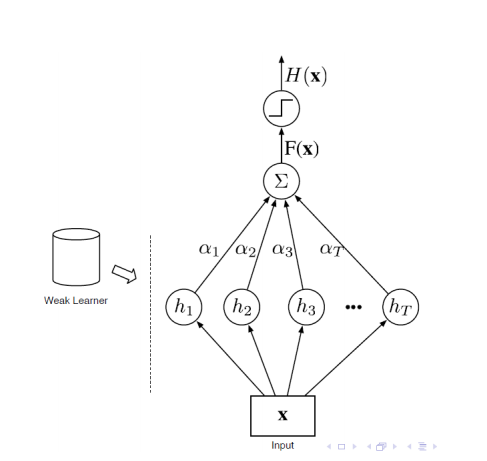
\includegraphics{img1.png}
\caption{schema}
\end{figure}

    \subsection{Training}\label{training}

At each iteration \(t\), a weak learner is generated and asigned a
coefficient \$ \alpha\_t \$ such that the sum training error \(E_t\) is
minimized.

\(E_ t = \sum{E[F_{t-1}(x_i) + \alpha_t h(x_i) ]}\)

The particularity of this method is that each weak classifier is trained
in order to better perform where the previous classifiers failed and
this is what makes this method really powerfull. In order to do this, at
each iteration of the training process, a weight \$ w\_\{i,t\}\$ is
assigned to each sample in the training set equal to the current error
\$ E(F\_\{t-1\}(x\_\{i\})) \$ on that sample. These weights are used to
inform the weak lerner were it has to focuse.

    \subsection{First experiments with
adaboost}\label{first-experiments-with-adaboost}

    In order to understand how Adaboost makes a prediction, we propose two
scenarios. The first one will use a dataset generated using
\textbf{sklearn datasets} and the second one will use a Pyrat dataset.
Let's generate clouds of points with 2 features, 1000 samples and 3
centers which represent the number of classes.

    \begin{Verbatim}[commandchars=\\\{\}]
{\color{incolor}In [{\color{incolor}85}]:} \PY{k+kn}{import} \PY{n+nn}{tqdm}
         \PY{k+kn}{import} \PY{n+nn}{numpy} \PY{k}{as} \PY{n+nn}{np}
         \PY{k+kn}{import} \PY{n+nn}{ast}
         \PY{k+kn}{import} \PY{n+nn}{os}
         \PY{k+kn}{from} \PY{n+nn}{sklearn}\PY{n+nn}{.}\PY{n+nn}{datasets} \PY{k}{import} \PY{n}{make\PYZus{}blobs}
         \PY{p}{[}\PY{n}{x}\PY{p}{,}\PY{n}{y}\PY{p}{]} \PY{o}{=} \PY{n}{make\PYZus{}blobs}\PY{p}{(}\PY{n}{n\PYZus{}samples}\PY{o}{=}\PY{l+m+mi}{1000}\PY{p}{,} \PY{n}{n\PYZus{}features}\PY{o}{=}\PY{l+m+mi}{2}\PY{p}{,} \PY{n}{centers}\PY{o}{=}\PY{l+m+mi}{3}\PY{p}{,}\PY{n}{random\PYZus{}state} \PY{o}{=} \PY{l+m+mi}{0}\PY{p}{)}
\end{Verbatim}


    \begin{Verbatim}[commandchars=\\\{\}]
{\color{incolor}In [{\color{incolor}6}]:} \PY{c+c1}{\PYZsh{}\PYZsh{}\PYZsh{} librarie to plot in python}
        \PY{k+kn}{import} \PY{n+nn}{matplotlib}\PY{n+nn}{.}\PY{n+nn}{pyplot} \PY{k}{as} \PY{n+nn}{plt}
        \PY{o}{\PYZpc{}}\PY{k}{matplotlib} inline
        \PY{n+nb}{print}\PY{p}{(}\PY{l+s+s2}{\PYZdq{}}\PY{l+s+s2}{Shape of dataset generated: }\PY{l+s+s2}{\PYZdq{}}\PY{p}{,} \PY{n}{x}\PY{o}{.}\PY{n}{shape}\PY{p}{)}
\end{Verbatim}


    \begin{Verbatim}[commandchars=\\\{\}]
Shape of dataset generated:  (1000, 2)

    \end{Verbatim}

    \begin{Verbatim}[commandchars=\\\{\}]
{\color{incolor}In [{\color{incolor}9}]:} \PY{n}{plt}\PY{o}{.}\PY{n}{scatter}\PY{p}{(}\PY{n}{x}\PY{p}{[}\PY{p}{:}\PY{p}{,}\PY{l+m+mi}{0}\PY{p}{]}\PY{p}{,}\PY{n}{x}\PY{p}{[}\PY{p}{:}\PY{p}{,}\PY{l+m+mi}{1}\PY{p}{]}\PY{p}{,}\PY{n}{c}\PY{o}{=}\PY{n}{y}\PY{p}{)}
        \PY{n}{plt}\PY{o}{.}\PY{n}{title}\PY{p}{(}\PY{l+s+s1}{\PYZsq{}}\PY{l+s+s1}{Input data}\PY{l+s+s1}{\PYZsq{}}\PY{p}{)}
\end{Verbatim}


\begin{Verbatim}[commandchars=\\\{\}]
{\color{outcolor}Out[{\color{outcolor}9}]:} Text(0.5, 1.0, 'Input data')
\end{Verbatim}
            
    \begin{center}
    \adjustimage{max size={0.9\linewidth}{0.9\paperheight}}{output_9_1.png}
    \end{center}
    { \hspace*{\fill} \\}
    
    In order to train and evaluate the classifier we are going to split the
dataset in 80\% train and 20\% test. We use random\_state = 0 so that
the function always returns the same split.

    \begin{Verbatim}[commandchars=\\\{\}]
{\color{incolor}In [{\color{incolor}86}]:} \PY{k+kn}{from} \PY{n+nn}{sklearn}\PY{n+nn}{.}\PY{n+nn}{model\PYZus{}selection} \PY{k}{import} \PY{n}{train\PYZus{}test\PYZus{}split}
         
         \PY{n}{x\PYZus{}train}\PY{p}{,}\PY{n}{x\PYZus{}test}\PY{p}{,}\PY{n}{y\PYZus{}train}\PY{p}{,}\PY{n}{y\PYZus{}test} \PY{o}{=} \PY{n}{train\PYZus{}test\PYZus{}split}\PY{p}{(}\PY{n}{x}\PY{p}{,}\PY{n}{y}\PY{p}{,}\PY{n}{random\PYZus{}state} \PY{o}{=} \PY{l+m+mi}{0}\PY{p}{,}\PY{n}{test\PYZus{}size}\PY{o}{=}\PY{l+m+mf}{0.2}\PY{p}{)}
         \PY{n+nb}{print}\PY{p}{(}\PY{l+s+s1}{\PYZsq{}}\PY{l+s+s1}{Training dataset shape : x}\PY{l+s+si}{\PYZob{}\PYZcb{}}\PY{l+s+s1}{, y}\PY{l+s+si}{\PYZob{}\PYZcb{}}\PY{l+s+s1}{\PYZsq{}}\PY{o}{.}\PY{n}{format}\PY{p}{(}\PY{n}{x\PYZus{}train}\PY{o}{.}\PY{n}{shape}\PY{p}{,}\PY{n}{y\PYZus{}train}\PY{o}{.}\PY{n}{shape}\PY{p}{)}\PY{p}{)}
         \PY{n+nb}{print}\PY{p}{(}\PY{l+s+s1}{\PYZsq{}}\PY{l+s+s1}{Test dataset shape : x}\PY{l+s+si}{\PYZob{}\PYZcb{}}\PY{l+s+s1}{, y}\PY{l+s+si}{\PYZob{}\PYZcb{}}\PY{l+s+s1}{\PYZsq{}}\PY{o}{.}\PY{n}{format}\PY{p}{(}\PY{n}{x\PYZus{}test}\PY{o}{.}\PY{n}{shape}\PY{p}{,}\PY{n}{y\PYZus{}test}\PY{o}{.}\PY{n}{shape}\PY{p}{)}\PY{p}{)}
\end{Verbatim}


    \begin{Verbatim}[commandchars=\\\{\}]
Training dataset shape : x(800, 2), y(800,)
Test dataset shape : x(200, 2), y(200,)

    \end{Verbatim}

    \begin{Verbatim}[commandchars=\\\{\}]
{\color{incolor}In [{\color{incolor}8}]:} \PY{c+c1}{\PYZsh{}function to plot boundaries}
        \PY{k+kn}{from} \PY{n+nn}{matplotlib}\PY{n+nn}{.}\PY{n+nn}{colors} \PY{k}{import} \PY{n}{ListedColormap}
        \PY{k+kn}{import} \PY{n+nn}{numpy} \PY{k}{as} \PY{n+nn}{np}
        \PY{k}{def} \PY{n+nf}{plot\PYZus{}boundaries}\PY{p}{(}\PY{n}{classifier}\PY{p}{,}\PY{n}{X}\PY{p}{,}\PY{n}{Y}\PY{p}{,}\PY{n}{ax}\PY{p}{,} \PY{n}{h}\PY{o}{=}\PY{l+m+mf}{0.2}\PY{p}{)}\PY{p}{:}
            \PY{n}{x0\PYZus{}min}\PY{p}{,} \PY{n}{x0\PYZus{}max} \PY{o}{=} \PY{n}{X}\PY{p}{[}\PY{p}{:}\PY{p}{,} \PY{l+m+mi}{0}\PY{p}{]}\PY{o}{.}\PY{n}{min}\PY{p}{(}\PY{p}{)} \PY{o}{\PYZhy{}} \PY{l+m+mi}{1}\PY{p}{,} \PY{n}{X}\PY{p}{[}\PY{p}{:}\PY{p}{,} \PY{l+m+mi}{0}\PY{p}{]}\PY{o}{.}\PY{n}{max}\PY{p}{(}\PY{p}{)} \PY{o}{+} \PY{l+m+mi}{1}
            \PY{n}{x1\PYZus{}min}\PY{p}{,} \PY{n}{x1\PYZus{}max} \PY{o}{=} \PY{n}{X}\PY{p}{[}\PY{p}{:}\PY{p}{,} \PY{l+m+mi}{1}\PY{p}{]}\PY{o}{.}\PY{n}{min}\PY{p}{(}\PY{p}{)} \PY{o}{\PYZhy{}} \PY{l+m+mi}{1}\PY{p}{,} \PY{n}{X}\PY{p}{[}\PY{p}{:}\PY{p}{,} \PY{l+m+mi}{1}\PY{p}{]}\PY{o}{.}\PY{n}{max}\PY{p}{(}\PY{p}{)} \PY{o}{+} \PY{l+m+mi}{1}
            \PY{n}{x0}\PY{p}{,} \PY{n}{x1} \PY{o}{=} \PY{n}{np}\PY{o}{.}\PY{n}{meshgrid}\PY{p}{(}\PY{n}{np}\PY{o}{.}\PY{n}{arange}\PY{p}{(}\PY{n}{x0\PYZus{}min}\PY{p}{,} \PY{n}{x0\PYZus{}max}\PY{p}{,}\PY{n}{h}\PY{p}{)}\PY{p}{,}
                                 \PY{n}{np}\PY{o}{.}\PY{n}{arange}\PY{p}{(}\PY{n}{x1\PYZus{}min}\PY{p}{,} \PY{n}{x1\PYZus{}max}\PY{p}{,}\PY{n}{h}\PY{p}{)}\PY{p}{)}
            \PY{n}{dataset} \PY{o}{=} \PY{n}{np}\PY{o}{.}\PY{n}{c\PYZus{}}\PY{p}{[}\PY{n}{x0}\PY{o}{.}\PY{n}{ravel}\PY{p}{(}\PY{p}{)}\PY{p}{,}\PY{n}{x1}\PY{o}{.}\PY{n}{ravel}\PY{p}{(}\PY{p}{)}\PY{p}{]}
            \PY{n}{Z} \PY{o}{=} \PY{n}{classifier}\PY{o}{.}\PY{n}{predict}\PY{p}{(}\PY{n}{dataset}\PY{p}{)}
        
            \PY{c+c1}{\PYZsh{} Put the result into a color plot}
            \PY{n}{Z} \PY{o}{=} \PY{n}{Z}\PY{o}{.}\PY{n}{reshape}\PY{p}{(}\PY{n}{x0}\PY{o}{.}\PY{n}{shape}\PY{p}{)}
            \PY{n}{ax}\PY{o}{.}\PY{n}{pcolormesh}\PY{p}{(}\PY{n}{x0}\PY{p}{,} \PY{n}{x1}\PY{p}{,} \PY{n}{Z}\PY{p}{)}
        
            \PY{c+c1}{\PYZsh{} Plot also the training points}
            \PY{n}{ax}\PY{o}{.}\PY{n}{scatter}\PY{p}{(}\PY{n}{X}\PY{p}{[}\PY{p}{:}\PY{p}{,} \PY{l+m+mi}{0}\PY{p}{]}\PY{p}{,} \PY{n}{X}\PY{p}{[}\PY{p}{:}\PY{p}{,} \PY{l+m+mi}{1}\PY{p}{]}\PY{p}{,} \PY{n}{c}\PY{o}{=}\PY{n}{Y}\PY{p}{,}
                        \PY{n}{edgecolor}\PY{o}{=}\PY{l+s+s1}{\PYZsq{}}\PY{l+s+s1}{k}\PY{l+s+s1}{\PYZsq{}}\PY{p}{,} \PY{n}{s}\PY{o}{=}\PY{l+m+mi}{20}\PY{p}{)}
            \PY{n}{ax}\PY{o}{.}\PY{n}{xlim}\PY{p}{(}\PY{n}{x0}\PY{o}{.}\PY{n}{min}\PY{p}{(}\PY{p}{)}\PY{p}{,} \PY{n}{x0}\PY{o}{.}\PY{n}{max}\PY{p}{(}\PY{p}{)}\PY{p}{)}
            \PY{n}{ax}\PY{o}{.}\PY{n}{ylim}\PY{p}{(}\PY{n}{x1}\PY{o}{.}\PY{n}{min}\PY{p}{(}\PY{p}{)}\PY{p}{,} \PY{n}{x1}\PY{o}{.}\PY{n}{max}\PY{p}{(}\PY{p}{)}\PY{p}{)}
\end{Verbatim}


    \subsubsection{Defining classifiers}\label{defining-classifiers}

    Let's use an Adaboost classifier to test whether we can classify this
data. To use it with sklearn we import the class
\href{https://scikit-learn.org/stable/modules/generated/sklearn.ensemble.AdaBoostClassifier.html\#sklearn.ensemble.AdaBoostClassifier}{AdaBoostClassifier}.
This class implements the algorithm known as Multi-class AdaBoost. We
are going to use \textbf{Decision Tree Classifier} as weak classifiers.
To see how Adaboost works we propose to increase the number of
estimators and see how it defines the boundaries each time.

    \begin{Verbatim}[commandchars=\\\{\}]
{\color{incolor}In [{\color{incolor}87}]:} \PY{k+kn}{from} \PY{n+nn}{sklearn}\PY{n+nn}{.}\PY{n+nn}{tree} \PY{k}{import} \PY{n}{DecisionTreeClassifier}
         \PY{k+kn}{from} \PY{n+nn}{sklearn}\PY{n+nn}{.}\PY{n+nn}{ensemble} \PY{k}{import} \PY{n}{AdaBoostClassifier}
         \PY{k+kn}{from} \PY{n+nn}{sklearn}\PY{n+nn}{.}\PY{n+nn}{metrics} \PY{k}{import} \PY{n}{accuracy\PYZus{}score}
         
         \PY{n}{classifiers}  \PY{o}{=} \PY{p}{[}\PY{n}{AdaBoostClassifier}\PY{p}{(}\PY{n}{DecisionTreeClassifier}\PY{p}{(}\PY{n}{max\PYZus{}depth}\PY{o}{=}\PY{l+m+mi}{1}\PY{p}{)}\PY{p}{,}\PY{n}{n\PYZus{}estimators}\PY{o}{=}\PY{l+m+mi}{1}\PY{p}{)}\PY{p}{,}
                         \PY{n}{AdaBoostClassifier}\PY{p}{(}\PY{n}{DecisionTreeClassifier}\PY{p}{(}\PY{n}{max\PYZus{}depth}\PY{o}{=}\PY{l+m+mi}{1}\PY{p}{)}\PY{p}{,}\PY{n}{n\PYZus{}estimators}\PY{o}{=}\PY{l+m+mi}{5}\PY{p}{)}\PY{p}{,}
                         \PY{n}{AdaBoostClassifier}\PY{p}{(}\PY{n}{DecisionTreeClassifier}\PY{p}{(}\PY{n}{max\PYZus{}depth}\PY{o}{=}\PY{l+m+mi}{1}\PY{p}{)}\PY{p}{,}\PY{n}{n\PYZus{}estimators}\PY{o}{=}\PY{l+m+mi}{10}\PY{p}{)}\PY{p}{,}
                         \PY{n}{AdaBoostClassifier}\PY{p}{(}\PY{n}{DecisionTreeClassifier}\PY{p}{(}\PY{n}{max\PYZus{}depth}\PY{o}{=}\PY{l+m+mi}{1}\PY{p}{)}\PY{p}{,}\PY{n}{n\PYZus{}estimators}\PY{o}{=}\PY{l+m+mi}{15}\PY{p}{)}\PY{p}{]}
         
         \PY{n}{fig} \PY{o}{=} \PY{n}{plt}\PY{o}{.}\PY{n}{figure}\PY{p}{(}\PY{n}{figsize}\PY{o}{=}\PY{p}{(}\PY{l+m+mi}{16}\PY{p}{,}\PY{l+m+mi}{10}\PY{p}{)}\PY{p}{)}
         
         
         \PY{c+c1}{\PYZsh{}\PYZhy{}\PYZhy{}\PYZhy{}\PYZhy{}\PYZhy{}\PYZhy{}\PYZhy{}\PYZhy{}\PYZhy{}\PYZhy{}\PYZhy{}\PYZhy{}\PYZhy{}\PYZhy{}\PYZhy{}\PYZhy{}\PYZhy{}\PYZhy{}\PYZhy{}\PYZhy{}\PYZhy{}\PYZhy{} Loop to make the graph from each desired classifier}
         \PY{k}{for} \PY{n}{i}\PY{p}{,}\PY{n}{clf} \PY{o+ow}{in} \PY{n+nb}{enumerate}\PY{p}{(}\PY{n}{classifiers}\PY{p}{)}\PY{p}{:}
             \PY{n}{ax} \PY{o}{=} \PY{n}{fig}\PY{o}{.}\PY{n}{add\PYZus{}subplot}\PY{p}{(}\PY{l+m+mi}{2}\PY{p}{,}\PY{l+m+mi}{4}\PY{p}{,}\PY{l+m+mi}{2}\PY{o}{*}\PY{n}{i} \PY{o}{+}\PY{l+m+mi}{1}\PY{p}{)} 
             \PY{n}{clf}\PY{o}{.}\PY{n}{fit}\PY{p}{(}\PY{n}{x\PYZus{}train}\PY{p}{,}\PY{n}{y\PYZus{}train}\PY{p}{)}
             \PY{n}{plot\PYZus{}boundaries}\PY{p}{(}\PY{n}{clf}\PY{p}{,}\PY{n}{x\PYZus{}train}\PY{p}{,}\PY{n}{y\PYZus{}train}\PY{p}{,}\PY{n}{plt}\PY{p}{)}
             
             \PY{c+c1}{\PYZsh{}\PYZhy{}\PYZhy{}\PYZhy{}\PYZhy{} evolution each classifier}
             \PY{n}{acc} \PY{o}{=} \PY{p}{[}\PY{p}{]}
             \PY{k}{for} \PY{n}{y\PYZus{}pred} \PY{o+ow}{in} \PY{n}{clf}\PY{o}{.}\PY{n}{staged\PYZus{}predict}\PY{p}{(}\PY{n}{x\PYZus{}test}\PY{p}{)}\PY{p}{:} 
                 \PY{n}{acc}\PY{o}{.}\PY{n}{append}\PY{p}{(}\PY{n}{accuracy\PYZus{}score}\PY{p}{(}\PY{n}{y\PYZus{}pred}\PY{p}{,} \PY{n}{y\PYZus{}test}\PY{p}{)}\PY{p}{)} \PY{c+c1}{\PYZsh{} \PYZhy{}\PYZhy{}\PYZhy{} test error each boosting stage}
             \PY{n}{n\PYZus{}trees} \PY{o}{=} \PY{n+nb}{len}\PY{p}{(}\PY{n}{clf}\PY{p}{)} \PY{c+c1}{\PYZsh{} : number where boosting was completed}
             
             \PY{n}{plt}\PY{o}{.}\PY{n}{title}\PY{p}{(}\PY{l+s+s1}{\PYZsq{}}\PY{l+s+s1}{Boundaries training \PYZsh{} }\PY{l+s+si}{\PYZob{}\PYZcb{}}\PY{l+s+s1}{ trees}\PY{l+s+s1}{\PYZsq{}}\PY{o}{.}\PY{n}{format}\PY{p}{(}\PY{n}{n\PYZus{}trees}\PY{p}{)}\PY{p}{)}
             \PY{n}{ax} \PY{o}{=} \PY{n}{fig}\PY{o}{.}\PY{n}{add\PYZus{}subplot}\PY{p}{(}\PY{l+m+mi}{2}\PY{p}{,}\PY{l+m+mi}{4}\PY{p}{,}\PY{n}{i}\PY{o}{*}\PY{l+m+mi}{2} \PY{o}{+}\PY{l+m+mi}{2}\PY{p}{)} 
             \PY{n}{plt}\PY{o}{.}\PY{n}{plot}\PY{p}{(}\PY{n+nb}{range}\PY{p}{(}\PY{l+m+mi}{1}\PY{p}{,} \PY{n}{n\PYZus{}trees} \PY{o}{+} \PY{l+m+mi}{1}\PY{p}{)}\PY{p}{,}\PY{n}{acc}\PY{p}{,}\PY{l+s+s1}{\PYZsq{}}\PY{l+s+s1}{.\PYZhy{}}\PY{l+s+s1}{\PYZsq{}}\PY{p}{)}
             \PY{n}{plt}\PY{o}{.}\PY{n}{title}\PY{p}{(}\PY{l+s+s1}{\PYZsq{}}\PY{l+s+s1}{Test accuracy }\PY{l+s+s1}{\PYZsq{}}\PY{p}{)}
             \PY{n}{plt}\PY{o}{.}\PY{n}{xlabel}\PY{p}{(}\PY{l+s+s1}{\PYZsq{}}\PY{l+s+s1}{Number of Trees}\PY{l+s+s1}{\PYZsq{}}\PY{p}{)}
         
         \PY{n}{plt}\PY{o}{.}\PY{n}{subplots\PYZus{}adjust}\PY{p}{(}\PY{n}{bottom}\PY{o}{=}\PY{l+m+mf}{0.15}\PY{p}{,} \PY{n}{wspace}\PY{o}{=}\PY{l+m+mf}{0.3}\PY{p}{)}
\end{Verbatim}


    \begin{center}
    \adjustimage{max size={0.9\linewidth}{0.9\paperheight}}{output_15_0.png}
    \end{center}
    { \hspace*{\fill} \\}
    
    As we can see in the figure above, the accuracy increases as the number
of estimators increases. This can also be seen in the boundary plot,
where the boundaries get better adapted to the training dataset when the
number of trees is incresead. However, if this number of trees is too
big, there could be overfitting.

    \section{Effect of the learning rate and the number of
trees}\label{effect-of-the-learning-rate-and-the-number-of-trees}

    In the following section, we are going to compare the accuracy of three
AdaBoosts (with different learning rates) while the number of trees
increases. The learning rate shrinks the contribution of each
classifier. We also compare these accuracies with those of simple
decision trees (with maximum depth of 1 and 2).

    We define the different AdaBoosts:

    \begin{Verbatim}[commandchars=\\\{\}]
{\color{incolor}In [{\color{incolor}89}]:} \PY{n}{clf\PYZus{}ada} \PY{o}{=} \PY{p}{[}\PY{n}{AdaBoostClassifier}\PY{p}{(}\PY{n}{DecisionTreeClassifier}\PY{p}{(}\PY{n}{max\PYZus{}depth}\PY{o}{=}\PY{l+m+mi}{1}\PY{p}{)}\PY{p}{,}\PY{n}{n\PYZus{}estimators}\PY{o}{=}\PY{l+m+mi}{200}\PY{p}{,}\PY{n}{learning\PYZus{}rate}\PY{o}{=}\PY{l+m+mf}{0.01}\PY{p}{)}\PY{p}{,}
                      \PY{n}{AdaBoostClassifier}\PY{p}{(}\PY{n}{DecisionTreeClassifier}\PY{p}{(}\PY{n}{max\PYZus{}depth}\PY{o}{=}\PY{l+m+mi}{1}\PY{p}{)}\PY{p}{,}\PY{n}{n\PYZus{}estimators}\PY{o}{=}\PY{l+m+mi}{200}\PY{p}{,}\PY{n}{learning\PYZus{}rate}\PY{o}{=}\PY{l+m+mf}{0.1}\PY{p}{)}\PY{p}{,}
                      \PY{n}{AdaBoostClassifier}\PY{p}{(}\PY{n}{DecisionTreeClassifier}\PY{p}{(}\PY{n}{max\PYZus{}depth}\PY{o}{=}\PY{l+m+mi}{1}\PY{p}{)}\PY{p}{,}\PY{n}{n\PYZus{}estimators}\PY{o}{=}\PY{l+m+mi}{200}\PY{p}{,}\PY{n}{learning\PYZus{}rate}\PY{o}{=}\PY{l+m+mf}{0.7}\PY{p}{)}\PY{p}{]}
         
         \PY{n}{test} \PY{o}{=} \PY{p}{[}\PY{p}{]}
         \PY{k}{for} \PY{n}{i}\PY{p}{,}\PY{n}{clf} \PY{o+ow}{in} \PY{n+nb}{enumerate}\PY{p}{(}\PY{n}{clf\PYZus{}ada}\PY{p}{)}\PY{p}{:}
             \PY{n}{clf}\PY{o}{.}\PY{n}{fit}\PY{p}{(}\PY{n}{x\PYZus{}train}\PY{p}{,}\PY{n}{y\PYZus{}train}\PY{p}{)}    
             \PY{c+c1}{\PYZsh{}\PYZhy{}\PYZhy{}\PYZhy{}\PYZhy{} evolution each classifier}
             \PY{n}{test\PYZus{}error} \PY{o}{=} \PY{p}{[}\PY{p}{]}
             \PY{k}{for} \PY{n}{y\PYZus{}pred} \PY{o+ow}{in} \PY{n}{clf}\PY{o}{.}\PY{n}{staged\PYZus{}predict}\PY{p}{(}\PY{n}{x\PYZus{}test}\PY{p}{)}\PY{p}{:} 
                 \PY{n}{test\PYZus{}error}\PY{o}{.}\PY{n}{append}\PY{p}{(}\PY{n}{accuracy\PYZus{}score}\PY{p}{(}\PY{n}{y\PYZus{}pred}\PY{p}{,} \PY{n}{y\PYZus{}test}\PY{p}{)}\PY{p}{)} \PY{c+c1}{\PYZsh{} \PYZhy{}\PYZhy{}\PYZhy{} test error each boosting stage    }
             \PY{n}{test}\PY{o}{.}\PY{n}{append}\PY{p}{(}\PY{n}{test\PYZus{}error}\PY{p}{)}
         
             
\end{Verbatim}


    We define the two decision trees:

    \begin{Verbatim}[commandchars=\\\{\}]
{\color{incolor}In [{\color{incolor}90}]:} \PY{n}{clf\PYZus{}tree} \PY{o}{=} \PY{p}{[}\PY{n}{DecisionTreeClassifier}\PY{p}{(}\PY{n}{max\PYZus{}depth}\PY{o}{=}\PY{l+m+mi}{1}\PY{p}{)}\PY{p}{,}
                    \PY{n}{DecisionTreeClassifier}\PY{p}{(}\PY{n}{max\PYZus{}depth}\PY{o}{=}\PY{l+m+mi}{2}\PY{p}{)}\PY{p}{]}
         \PY{k}{for} \PY{n}{i}\PY{p}{,}\PY{n}{clf} \PY{o+ow}{in} \PY{n+nb}{enumerate}\PY{p}{(}\PY{n}{clf\PYZus{}tree}\PY{p}{)}\PY{p}{:}
             \PY{n}{clf}\PY{o}{.}\PY{n}{fit}\PY{p}{(}\PY{n}{x\PYZus{}train}\PY{p}{,}\PY{n}{y\PYZus{}train}\PY{p}{)}    
             \PY{c+c1}{\PYZsh{}\PYZhy{}\PYZhy{}\PYZhy{}\PYZhy{} evolution each classifier}
             \PY{n}{test}\PY{o}{.}\PY{n}{append}\PY{p}{(}\PY{n}{clf}\PY{o}{.}\PY{n}{score}\PY{p}{(}\PY{n}{x\PYZus{}test}\PY{p}{,} \PY{n}{y\PYZus{}test}\PY{p}{)}\PY{o}{*}\PY{n}{np}\PY{o}{.}\PY{n}{ones}\PY{p}{(}\PY{l+m+mi}{200}\PY{p}{)}\PY{p}{)} \PY{c+c1}{\PYZsh{} \PYZhy{}\PYZhy{}\PYZhy{}}
\end{Verbatim}


    We make the comparaisons:

    \begin{Verbatim}[commandchars=\\\{\}]
{\color{incolor}In [{\color{incolor}91}]:} \PY{n}{fig} \PY{o}{=} \PY{n}{plt}\PY{o}{.}\PY{n}{figure}\PY{p}{(}\PY{n}{figsize}\PY{o}{=}\PY{p}{(}\PY{l+m+mi}{10}\PY{p}{,}\PY{l+m+mi}{6}\PY{p}{)}\PY{p}{)}
         \PY{n}{c} \PY{o}{=} \PY{p}{[}\PY{l+s+s1}{\PYZsq{}}\PY{l+s+s1}{\PYZhy{}}\PY{l+s+s1}{\PYZsq{}}\PY{p}{,}\PY{l+s+s1}{\PYZsq{}}\PY{l+s+s1}{\PYZhy{}}\PY{l+s+s1}{\PYZsq{}}\PY{p}{,}\PY{l+s+s1}{\PYZsq{}}\PY{l+s+s1}{\PYZhy{}}\PY{l+s+s1}{\PYZsq{}}\PY{p}{,}\PY{l+s+s1}{\PYZsq{}}\PY{l+s+s1}{\PYZhy{}\PYZhy{}}\PY{l+s+s1}{\PYZsq{}}\PY{p}{,}\PY{l+s+s1}{\PYZsq{}}\PY{l+s+s1}{\PYZhy{}\PYZhy{}}\PY{l+s+s1}{\PYZsq{}}\PY{p}{]}
         \PY{k}{for} \PY{n}{i}\PY{p}{,}\PY{n}{l} \PY{o+ow}{in} \PY{n+nb}{zip}\PY{p}{(}\PY{n}{test}\PY{p}{,}\PY{n}{c}\PY{p}{)}\PY{p}{:}
             \PY{n}{plt}\PY{o}{.}\PY{n}{plot}\PY{p}{(}\PY{n+nb}{range}\PY{p}{(}\PY{l+m+mi}{1}\PY{p}{,}\PY{l+m+mi}{201}\PY{p}{)}\PY{p}{,}\PY{n}{i}\PY{p}{,}\PY{n}{l}\PY{p}{)}
             
         \PY{n}{plt}\PY{o}{.}\PY{n}{legend}\PY{p}{(}\PY{p}{[}\PY{l+s+s1}{\PYZsq{}}\PY{l+s+s1}{Adaboost Accuracy LR=0.01}\PY{l+s+s1}{\PYZsq{}}\PY{p}{,}
                     \PY{l+s+s1}{\PYZsq{}}\PY{l+s+s1}{Adaboost Accuracy LR=0.1}\PY{l+s+s1}{\PYZsq{}}\PY{p}{,}
                     \PY{l+s+s1}{\PYZsq{}}\PY{l+s+s1}{Adaboost Accuracy LR=0.7}\PY{l+s+s1}{\PYZsq{}}\PY{p}{,}
                     \PY{l+s+s1}{\PYZsq{}}\PY{l+s+s1}{Decision Tree Accuracy depth = 1}\PY{l+s+s1}{\PYZsq{}}\PY{p}{,}
                     \PY{l+s+s1}{\PYZsq{}}\PY{l+s+s1}{Decision Tree Accuracy depth = 2}\PY{l+s+s1}{\PYZsq{}}\PY{p}{]}\PY{p}{)}
         \PY{n}{plt}\PY{o}{.}\PY{n}{ylabel}\PY{p}{(}\PY{l+s+s1}{\PYZsq{}}\PY{l+s+s1}{Test Accuracy}\PY{l+s+s1}{\PYZsq{}}\PY{p}{)}
         \PY{n}{plt}\PY{o}{.}\PY{n}{xlabel}\PY{p}{(}\PY{l+s+s1}{\PYZsq{}}\PY{l+s+s1}{Number of estimators}\PY{l+s+s1}{\PYZsq{}}\PY{p}{)}
         
         \PY{n}{plt}\PY{o}{.}\PY{n}{grid}\PY{p}{(}\PY{p}{)}
\end{Verbatim}


    \begin{center}
    \adjustimage{max size={0.9\linewidth}{0.9\paperheight}}{output_24_0.png}
    \end{center}
    { \hspace*{\fill} \\}
    
    \textbf{Observations} * We can see that we the number of estimators is
one, the accuracy is the same of the decision tree of depth 1 * We also
can see that the accuracy when having more estimators IS NOT the same as
the decision tree of depth 2. This shows that the method is adapting
different trees of depth 1 and it is not equivalent to change the tree's
depth. * We can see that the learning rate has a direct effect in the
evolution of the accuracy. If it is too small, it will too many
estimator to increase the accuracy. If it is too big, the accuracy will
start oscillating when increasing the number of estimators.

    In order to study how the learning rate affects the boundaries of the
decision areas, we plot them in the figure below for 200 estimators.

    \begin{Verbatim}[commandchars=\\\{\}]
{\color{incolor}In [{\color{incolor}92}]:} \PY{n}{fig} \PY{o}{=} \PY{n}{plt}\PY{o}{.}\PY{n}{figure}\PY{p}{(}\PY{n}{figsize}\PY{o}{=}\PY{p}{(}\PY{l+m+mi}{15}\PY{p}{,}\PY{l+m+mi}{4}\PY{p}{)}\PY{p}{)}
         \PY{n}{l} \PY{o}{=} \PY{p}{[}\PY{l+s+s1}{\PYZsq{}}\PY{l+s+s1}{LR = 0.01}\PY{l+s+s1}{\PYZsq{}}\PY{p}{,}
             \PY{l+s+s1}{\PYZsq{}}\PY{l+s+s1}{LR = 0.1}\PY{l+s+s1}{\PYZsq{}}\PY{p}{,}
             \PY{l+s+s1}{\PYZsq{}}\PY{l+s+s1}{LR = 0.7}\PY{l+s+s1}{\PYZsq{}}\PY{p}{]}
         \PY{k}{for} \PY{n}{i}\PY{p}{,}\PY{n}{t} \PY{o+ow}{in} \PY{n+nb}{enumerate}\PY{p}{(}\PY{n}{clf\PYZus{}ada}\PY{p}{)}\PY{p}{:}
             \PY{n}{ax} \PY{o}{=} \PY{n}{fig}\PY{o}{.}\PY{n}{add\PYZus{}subplot}\PY{p}{(}\PY{l+m+mi}{1}\PY{p}{,}\PY{l+m+mi}{3}\PY{p}{,}\PY{n}{i}\PY{o}{+}\PY{l+m+mi}{1}\PY{p}{)}
             \PY{n}{plot\PYZus{}boundaries}\PY{p}{(}\PY{n}{t}\PY{p}{,}\PY{n}{x\PYZus{}train}\PY{p}{,}\PY{n}{y\PYZus{}train}\PY{p}{,}\PY{n}{plt}\PY{p}{)}
             \PY{n}{plt}\PY{o}{.}\PY{n}{xlabel}\PY{p}{(}\PY{n}{l}\PY{p}{[}\PY{n}{i}\PY{p}{]}\PY{p}{,}\PY{n}{size}\PY{o}{=}\PY{l+m+mi}{15}\PY{p}{)}
             
\end{Verbatim}


    \begin{center}
    \adjustimage{max size={0.9\linewidth}{0.9\paperheight}}{output_27_0.png}
    \end{center}
    { \hspace*{\fill} \\}
    
    It can be seen that, as the learning rate increases, the boundaries get
more complex. This may have a negative effect, has seen when LR=0,7.

    \section{Application to Pyrat}\label{application-to-pyrat}

    We apply this method to the problem of predicting the winner in the
Pyrat game. We consider the three posible ends as classes. python wins,
rat wins and draw.

    \begin{Verbatim}[commandchars=\\\{\}]
{\color{incolor}In [{\color{incolor}95}]:} \PY{n}{loaded\PYZus{}data} \PY{o}{=} \PY{n}{np}\PY{o}{.}\PY{n}{load}\PY{p}{(}\PY{l+s+s2}{\PYZdq{}}\PY{l+s+s2}{dataset.npz}\PY{l+s+s2}{\PYZdq{}}\PY{p}{)}
         \PY{n}{x\PYZus{}pyrat} \PY{o}{=} \PY{n}{loaded\PYZus{}data}\PY{p}{[}\PY{l+s+s2}{\PYZdq{}}\PY{l+s+s2}{x}\PY{l+s+s2}{\PYZdq{}}\PY{p}{]}
         \PY{n}{y\PYZus{}pyrat} \PY{o}{=} \PY{n}{loaded\PYZus{}data}\PY{p}{[}\PY{l+s+s2}{\PYZdq{}}\PY{l+s+s2}{y}\PY{l+s+s2}{\PYZdq{}}\PY{p}{]}
\end{Verbatim}


    \begin{Verbatim}[commandchars=\\\{\}]
{\color{incolor}In [{\color{incolor}96}]:} \PY{n+nb}{print}\PY{p}{(}\PY{l+s+s2}{\PYZdq{}}\PY{l+s+s2}{Input data shape:x}\PY{l+s+si}{\PYZob{}\PYZcb{}}\PY{l+s+s2}{,y}\PY{l+s+si}{\PYZob{}\PYZcb{}}\PY{l+s+s2}{\PYZdq{}}\PY{o}{.}\PY{n}{format}\PY{p}{(}\PY{n}{x\PYZus{}pyrat}\PY{o}{.}\PY{n}{shape}\PY{p}{,}\PY{n}{y\PYZus{}pyrat}\PY{o}{.}\PY{n}{shape}\PY{p}{)}\PY{p}{)}
\end{Verbatim}


    \begin{Verbatim}[commandchars=\\\{\}]
Input data shape:x(1000, 315),y(1000,)

    \end{Verbatim}

    \begin{Verbatim}[commandchars=\\\{\}]
{\color{incolor}In [{\color{incolor}97}]:} \PY{n}{x\PYZus{}train}\PY{p}{,}\PY{n}{x\PYZus{}test}\PY{p}{,}\PY{n}{y\PYZus{}train}\PY{p}{,}\PY{n}{y\PYZus{}test} \PY{o}{=} \PY{n}{train\PYZus{}test\PYZus{}split}\PY{p}{(}\PY{n}{x\PYZus{}pyrat}\PY{p}{,}\PY{n}{y\PYZus{}pyrat}\PY{p}{,}\PY{n}{random\PYZus{}state} \PY{o}{=} \PY{l+m+mi}{0}\PY{p}{,}\PY{n}{test\PYZus{}size}\PY{o}{=}\PY{l+m+mf}{0.2}\PY{p}{)}
         \PY{n+nb}{print}\PY{p}{(}\PY{l+s+s1}{\PYZsq{}}\PY{l+s+s1}{Training dataset shape : x}\PY{l+s+si}{\PYZob{}\PYZcb{}}\PY{l+s+s1}{, y}\PY{l+s+si}{\PYZob{}\PYZcb{}}\PY{l+s+s1}{\PYZsq{}}\PY{o}{.}\PY{n}{format}\PY{p}{(}\PY{n}{x\PYZus{}train}\PY{o}{.}\PY{n}{shape}\PY{p}{,}\PY{n}{y\PYZus{}train}\PY{o}{.}\PY{n}{shape}\PY{p}{)}\PY{p}{)}
         \PY{n+nb}{print}\PY{p}{(}\PY{l+s+s1}{\PYZsq{}}\PY{l+s+s1}{Test dataset shape : x}\PY{l+s+si}{\PYZob{}\PYZcb{}}\PY{l+s+s1}{, y}\PY{l+s+si}{\PYZob{}\PYZcb{}}\PY{l+s+s1}{\PYZsq{}}\PY{o}{.}\PY{n}{format}\PY{p}{(}\PY{n}{x\PYZus{}test}\PY{o}{.}\PY{n}{shape}\PY{p}{,}\PY{n}{y\PYZus{}test}\PY{o}{.}\PY{n}{shape}\PY{p}{)}\PY{p}{)}
\end{Verbatim}


    \begin{Verbatim}[commandchars=\\\{\}]
Training dataset shape : x(800, 315), y(800,)
Test dataset shape : x(200, 315), y(200,)

    \end{Verbatim}

    \begin{Verbatim}[commandchars=\\\{\}]
{\color{incolor}In [{\color{incolor}98}]:} \PY{n}{clf\PYZus{}py} \PY{o}{=} \PY{n}{AdaBoostClassifier}\PY{p}{(}\PY{n}{DecisionTreeClassifier}\PY{p}{(}\PY{n}{max\PYZus{}depth}\PY{o}{=}\PY{l+m+mi}{1}\PY{p}{)}\PY{p}{,}\PY{n}{n\PYZus{}estimators}\PY{o}{=}\PY{l+m+mi}{100}\PY{p}{,}\PY{n}{learning\PYZus{}rate}\PY{o}{=}\PY{l+m+mf}{0.05}\PY{p}{)}
         \PY{n}{clf\PYZus{}py}\PY{o}{.}\PY{n}{fit}\PY{p}{(}\PY{n}{x\PYZus{}train}\PY{p}{,}\PY{n}{y\PYZus{}train}\PY{p}{)}    
             \PY{c+c1}{\PYZsh{}\PYZhy{}\PYZhy{}\PYZhy{}\PYZhy{} evolution each classifier}
         \PY{n}{test\PYZus{}error} \PY{o}{=} \PY{p}{[}\PY{p}{]}
         \PY{k}{for} \PY{n}{y\PYZus{}pred} \PY{o+ow}{in} \PY{n}{clf\PYZus{}py}\PY{o}{.}\PY{n}{staged\PYZus{}predict}\PY{p}{(}\PY{n}{x\PYZus{}test}\PY{p}{)}\PY{p}{:} 
             \PY{n}{test\PYZus{}error}\PY{o}{.}\PY{n}{append}\PY{p}{(}\PY{n}{accuracy\PYZus{}score}\PY{p}{(}\PY{n}{y\PYZus{}pred}\PY{p}{,} \PY{n}{y\PYZus{}test}\PY{p}{)}\PY{p}{)} \PY{c+c1}{\PYZsh{} \PYZhy{}\PYZhy{}\PYZhy{} test error each boosting stage    }
\end{Verbatim}


    \begin{Verbatim}[commandchars=\\\{\}]
{\color{incolor}In [{\color{incolor}99}]:} \PY{n+nb}{print}\PY{p}{(}\PY{l+s+s2}{\PYZdq{}}\PY{l+s+s2}{Accuracy on the training set }\PY{l+s+si}{\PYZob{}\PYZcb{}}\PY{l+s+s2}{\PYZpc{}}\PY{l+s+s2}{\PYZdq{}}\PY{o}{.}\PY{n}{format}\PY{p}{(}\PY{n}{clf\PYZus{}py}\PY{o}{.}\PY{n}{score}\PY{p}{(}\PY{n}{x\PYZus{}train}\PY{p}{,}\PY{n}{y\PYZus{}train}\PY{p}{)}\PY{o}{*}\PY{l+m+mi}{100}\PY{p}{)}\PY{p}{)}
         \PY{n+nb}{print}\PY{p}{(}\PY{l+s+s2}{\PYZdq{}}\PY{l+s+s2}{Accuracy on the test set }\PY{l+s+si}{\PYZob{}\PYZcb{}}\PY{l+s+s2}{\PYZpc{}}\PY{l+s+s2}{\PYZdq{}}\PY{o}{.}\PY{n}{format}\PY{p}{(}\PY{n}{clf\PYZus{}py}\PY{o}{.}\PY{n}{score}\PY{p}{(}\PY{n}{x\PYZus{}test}\PY{p}{,}\PY{n}{y\PYZus{}test}\PY{p}{)}\PY{o}{*}\PY{l+m+mi}{100}\PY{p}{)}\PY{p}{)}
\end{Verbatim}


    \begin{Verbatim}[commandchars=\\\{\}]
Accuracy on the training set 52.87500000000001\%
Accuracy on the test set 50.5\%

    \end{Verbatim}

    We calculate the confusion matrix.

    \begin{Verbatim}[commandchars=\\\{\}]
{\color{incolor}In [{\color{incolor}100}]:} \PY{k+kn}{from} \PY{n+nn}{sklearn}\PY{n+nn}{.}\PY{n+nn}{metrics} \PY{k}{import} \PY{n}{classification\PYZus{}report}\PY{p}{,}\PY{n}{confusion\PYZus{}matrix}
          \PY{n}{y\PYZus{}pred\PYZus{}train} \PY{o}{=} \PY{n}{clf\PYZus{}py}\PY{o}{.}\PY{n}{predict}\PY{p}{(}\PY{n}{x\PYZus{}train}\PY{p}{)}
          \PY{n}{report} \PY{o}{=} \PY{n}{classification\PYZus{}report}\PY{p}{(}\PY{n}{y\PYZus{}true}\PY{o}{=}\PY{n}{y\PYZus{}train}\PY{p}{,}\PY{n}{y\PYZus{}pred}\PY{o}{=}\PY{n}{y\PYZus{}pred\PYZus{}train}\PY{p}{)}
          \PY{n}{matrix} \PY{o}{=} \PY{n}{confusion\PYZus{}matrix}\PY{p}{(}\PY{n}{y\PYZus{}true}\PY{o}{=}\PY{n}{y\PYZus{}train}\PY{p}{,}\PY{n}{y\PYZus{}pred}\PY{o}{=}\PY{n}{y\PYZus{}pred\PYZus{}train}\PY{p}{)}
          \PY{n+nb}{print}\PY{p}{(}\PY{l+s+s2}{\PYZdq{}}\PY{l+s+s2}{Training Set:}\PY{l+s+s2}{\PYZdq{}}\PY{p}{)}
          \PY{n+nb}{print}\PY{p}{(}\PY{n}{report}\PY{p}{)}
          \PY{n+nb}{print}\PY{p}{(}\PY{n}{matrix}\PY{p}{)}
          \PY{n}{plt}\PY{o}{.}\PY{n}{matshow}\PY{p}{(}\PY{n}{matrix}\PY{p}{)}
          \PY{n}{plt}\PY{o}{.}\PY{n}{colorbar}\PY{p}{(}\PY{p}{)}
          
          \PY{n}{plt}\PY{o}{.}\PY{n}{xlabel}\PY{p}{(}\PY{l+s+s2}{\PYZdq{}}\PY{l+s+s2}{Predicted Class}\PY{l+s+s2}{\PYZdq{}}\PY{p}{)}
          \PY{n}{plt}\PY{o}{.}\PY{n}{ylabel}\PY{p}{(}\PY{l+s+s2}{\PYZdq{}}\PY{l+s+s2}{Real Class}\PY{l+s+s2}{\PYZdq{}}\PY{p}{)}
\end{Verbatim}


    \begin{Verbatim}[commandchars=\\\{\}]
Training Set:
             precision    recall  f1-score   support

       -1.0       0.54      0.50      0.52       342
        0.0       0.00      0.00      0.00       101
        1.0       0.52      0.71      0.60       357

avg / total       0.46      0.53      0.49       800

[[170   0 172]
 [ 43   0  58]
 [104   0 253]]

    \end{Verbatim}

    \begin{Verbatim}[commandchars=\\\{\}]
/home/brain/miniconda3/lib/python3.6/site-packages/sklearn/metrics/classification.py:1135: UndefinedMetricWarning: Precision and F-score are ill-defined and being set to 0.0 in labels with no predicted samples.
  'precision', 'predicted', average, warn\_for)

    \end{Verbatim}

\begin{Verbatim}[commandchars=\\\{\}]
{\color{outcolor}Out[{\color{outcolor}100}]:} Text(0,0.5,'Real Class')
\end{Verbatim}
            
    \begin{center}
    \adjustimage{max size={0.9\linewidth}{0.9\paperheight}}{output_37_3.png}
    \end{center}
    { \hspace*{\fill} \\}
    
    We can see that the main problem is in the second class, the draw. As we
can see, this is possibly due to the fact that the number of samples is
too small.

    \begin{Verbatim}[commandchars=\\\{\}]
{\color{incolor}In [{\color{incolor}111}]:} \PY{n}{rat\PYZus{}win\PYZus{}index} \PY{o}{=} \PY{n}{y\PYZus{}train} \PY{o}{==} \PY{o}{\PYZhy{}}\PY{l+m+mi}{1}
          \PY{n}{draw\PYZus{}index} \PY{o}{=} \PY{n}{y\PYZus{}train} \PY{o}{==} \PY{l+m+mi}{0}
          \PY{n}{python\PYZus{}win\PYZus{}index} \PY{o}{=} \PY{n}{y\PYZus{}train} \PY{o}{==} \PY{l+m+mi}{1}
          
          \PY{n+nb}{print}\PY{p}{(}\PY{l+s+s1}{\PYZsq{}}\PY{l+s+s1}{Training draw: }\PY{l+s+si}{\PYZob{}\PYZcb{}}\PY{l+s+s1}{,Training rat wins: }\PY{l+s+si}{\PYZob{}\PYZcb{}}\PY{l+s+s1}{,Training python wins: }\PY{l+s+si}{\PYZob{}\PYZcb{}}\PY{l+s+s1}{\PYZsq{}}\PY{o}{.}\PY{n}{format}\PY{p}{(}\PY{n+nb}{len}\PY{p}{(}\PY{n}{y\PYZus{}train}\PY{p}{[}\PY{n}{draw\PYZus{}index}\PY{p}{]}\PY{p}{)}\PY{p}{,}\PY{n+nb}{len}\PY{p}{(}\PY{n}{y\PYZus{}train}\PY{p}{[}\PY{n}{rat\PYZus{}win\PYZus{}index}\PY{p}{]}\PY{p}{)}\PY{p}{,}\PY{n+nb}{len}\PY{p}{(}\PY{n}{y\PYZus{}train}\PY{p}{[}\PY{n}{python\PYZus{}win\PYZus{}index}\PY{p}{]}\PY{p}{)}\PY{p}{)}\PY{p}{)}
          
          \PY{n+nb}{print}\PY{p}{(}\PY{l+s+s1}{\PYZsq{}}\PY{l+s+s1}{Test draw: }\PY{l+s+si}{\PYZob{}\PYZcb{}}\PY{l+s+s1}{,Test rat wins: }\PY{l+s+si}{\PYZob{}\PYZcb{}}\PY{l+s+s1}{,Test python wins: }\PY{l+s+si}{\PYZob{}\PYZcb{}}\PY{l+s+s1}{\PYZsq{}}\PY{o}{.}\PY{n}{format}\PY{p}{(}\PY{n+nb}{len}\PY{p}{(}\PY{n}{y\PYZus{}test}\PY{p}{[}\PY{n}{y\PYZus{}test} \PY{o}{==} \PY{l+m+mi}{0}\PY{p}{]}\PY{p}{)}\PY{p}{,}\PY{n+nb}{len}\PY{p}{(}\PY{n}{y\PYZus{}test}\PY{p}{[}\PY{n}{y\PYZus{}test} \PY{o}{==} \PY{o}{\PYZhy{}}\PY{l+m+mi}{1} \PY{p}{]}\PY{p}{)}\PY{p}{,}\PY{n+nb}{len}\PY{p}{(}\PY{n}{y\PYZus{}test}\PY{p}{[}\PY{n}{y\PYZus{}test}\PY{o}{==}\PY{l+m+mi}{1}\PY{p}{]}\PY{p}{)}\PY{p}{)}\PY{p}{)}
\end{Verbatim}


    \begin{Verbatim}[commandchars=\\\{\}]
Training draw: 101,Training rat wins: 342,Training python wins: 357
Test draw: 19,Test rat wins: 84,Test python wins: 97

    \end{Verbatim}

    \subsection{Binary classification}\label{binary-classification}

We perform now a binary classification between the classes python and
rat wins (we don't consider anymore the draws).

    \begin{Verbatim}[commandchars=\\\{\}]
{\color{incolor}In [{\color{incolor}115}]:} \PY{c+c1}{\PYZsh{}\PYZsh{} binary classification}
          \PY{n}{x\PYZus{}p} \PY{o}{=} \PY{p}{[}\PY{p}{]}
          \PY{n}{y\PYZus{}p} \PY{o}{=} \PY{p}{[}\PY{p}{]}
          \PY{k}{for} \PY{n}{x}\PY{p}{,}\PY{n}{y} \PY{o+ow}{in} \PY{n+nb}{zip}\PY{p}{(}\PY{n}{x\PYZus{}pyrat}\PY{p}{,}\PY{n}{y\PYZus{}pyrat}\PY{p}{)}\PY{p}{:}
              \PY{k}{if} \PY{n}{y} \PY{o}{!=} \PY{l+m+mi}{0}\PY{p}{:}
                  \PY{n}{x\PYZus{}p}\PY{o}{.}\PY{n}{append}\PY{p}{(}\PY{n}{x}\PY{p}{)}
                  \PY{n}{y\PYZus{}p}\PY{o}{.}\PY{n}{append}\PY{p}{(}\PY{n}{y}\PY{p}{)}
          \PY{n}{x\PYZus{}pyrat\PYZus{}b} \PY{o}{=} \PY{n}{np}\PY{o}{.}\PY{n}{asarray}\PY{p}{(}\PY{n}{x\PYZus{}p}\PY{p}{)}
          \PY{n}{y\PYZus{}pyrat\PYZus{}b} \PY{o}{=} \PY{n}{np}\PY{o}{.}\PY{n}{asarray}\PY{p}{(}\PY{n}{y\PYZus{}p}\PY{p}{)}
\end{Verbatim}


    \begin{Verbatim}[commandchars=\\\{\}]
{\color{incolor}In [{\color{incolor}116}]:} \PY{n}{x\PYZus{}train}\PY{p}{,}\PY{n}{x\PYZus{}test}\PY{p}{,}\PY{n}{y\PYZus{}train}\PY{p}{,}\PY{n}{y\PYZus{}test} \PY{o}{=} \PY{n}{train\PYZus{}test\PYZus{}split}\PY{p}{(}\PY{n}{x\PYZus{}pyrat\PYZus{}b}\PY{p}{,}\PY{n}{y\PYZus{}pyrat\PYZus{}b}\PY{p}{,}\PY{n}{random\PYZus{}state} \PY{o}{=} \PY{l+m+mi}{0}\PY{p}{,}\PY{n}{test\PYZus{}size}\PY{o}{=}\PY{l+m+mf}{0.2}\PY{p}{)}
          \PY{n+nb}{print}\PY{p}{(}\PY{l+s+s1}{\PYZsq{}}\PY{l+s+s1}{Training dataset shape : x}\PY{l+s+si}{\PYZob{}\PYZcb{}}\PY{l+s+s1}{, y}\PY{l+s+si}{\PYZob{}\PYZcb{}}\PY{l+s+s1}{\PYZsq{}}\PY{o}{.}\PY{n}{format}\PY{p}{(}\PY{n}{x\PYZus{}train}\PY{o}{.}\PY{n}{shape}\PY{p}{,}\PY{n}{y\PYZus{}train}\PY{o}{.}\PY{n}{shape}\PY{p}{)}\PY{p}{)}
          \PY{n+nb}{print}\PY{p}{(}\PY{l+s+s1}{\PYZsq{}}\PY{l+s+s1}{Test dataset shape : x}\PY{l+s+si}{\PYZob{}\PYZcb{}}\PY{l+s+s1}{, y}\PY{l+s+si}{\PYZob{}\PYZcb{}}\PY{l+s+s1}{\PYZsq{}}\PY{o}{.}\PY{n}{format}\PY{p}{(}\PY{n}{x\PYZus{}test}\PY{o}{.}\PY{n}{shape}\PY{p}{,}\PY{n}{y\PYZus{}test}\PY{o}{.}\PY{n}{shape}\PY{p}{)}\PY{p}{)}
\end{Verbatim}


    \begin{Verbatim}[commandchars=\\\{\}]
Training dataset shape : x(704, 315), y(704,)
Test dataset shape : x(176, 315), y(176,)

    \end{Verbatim}

    \begin{Verbatim}[commandchars=\\\{\}]
{\color{incolor}In [{\color{incolor}117}]:} \PY{n}{clf\PYZus{}py} \PY{o}{=} \PY{n}{AdaBoostClassifier}\PY{p}{(}\PY{n}{DecisionTreeClassifier}\PY{p}{(}\PY{n}{max\PYZus{}depth}\PY{o}{=}\PY{l+m+mi}{1}\PY{p}{)}\PY{p}{,}\PY{n}{n\PYZus{}estimators}\PY{o}{=}\PY{l+m+mi}{100}\PY{p}{,}\PY{n}{learning\PYZus{}rate}\PY{o}{=}\PY{l+m+mf}{0.05}\PY{p}{)}
          \PY{n}{clf\PYZus{}py}\PY{o}{.}\PY{n}{fit}\PY{p}{(}\PY{n}{x\PYZus{}train}\PY{p}{,}\PY{n}{y\PYZus{}train}\PY{p}{)}    
              \PY{c+c1}{\PYZsh{}\PYZhy{}\PYZhy{}\PYZhy{}\PYZhy{} evolution each classifier}
          \PY{n}{test\PYZus{}error} \PY{o}{=} \PY{p}{[}\PY{p}{]}
          \PY{k}{for} \PY{n}{y\PYZus{}pred} \PY{o+ow}{in} \PY{n}{clf\PYZus{}py}\PY{o}{.}\PY{n}{staged\PYZus{}predict}\PY{p}{(}\PY{n}{x\PYZus{}test}\PY{p}{)}\PY{p}{:} 
              \PY{n}{test\PYZus{}error}\PY{o}{.}\PY{n}{append}\PY{p}{(}\PY{n}{accuracy\PYZus{}score}\PY{p}{(}\PY{n}{y\PYZus{}pred}\PY{p}{,} \PY{n}{y\PYZus{}test}\PY{p}{)}\PY{p}{)} \PY{c+c1}{\PYZsh{} \PYZhy{}\PYZhy{}\PYZhy{} test error each boosting stage    }
\end{Verbatim}


    \begin{Verbatim}[commandchars=\\\{\}]
{\color{incolor}In [{\color{incolor}118}]:} \PY{n+nb}{print}\PY{p}{(}\PY{l+s+s2}{\PYZdq{}}\PY{l+s+s2}{Accuracy on the training set }\PY{l+s+si}{\PYZob{}\PYZcb{}}\PY{l+s+s2}{\PYZpc{}}\PY{l+s+s2}{\PYZdq{}}\PY{o}{.}\PY{n}{format}\PY{p}{(}\PY{n}{clf\PYZus{}py}\PY{o}{.}\PY{n}{score}\PY{p}{(}\PY{n}{x\PYZus{}train}\PY{p}{,}\PY{n}{y\PYZus{}train}\PY{p}{)}\PY{o}{*}\PY{l+m+mi}{100}\PY{p}{)}\PY{p}{)}
          \PY{n+nb}{print}\PY{p}{(}\PY{l+s+s2}{\PYZdq{}}\PY{l+s+s2}{Accuracy on the test set }\PY{l+s+si}{\PYZob{}\PYZcb{}}\PY{l+s+s2}{\PYZpc{}}\PY{l+s+s2}{\PYZdq{}}\PY{o}{.}\PY{n}{format}\PY{p}{(}\PY{n}{clf\PYZus{}py}\PY{o}{.}\PY{n}{score}\PY{p}{(}\PY{n}{x\PYZus{}test}\PY{p}{,}\PY{n}{y\PYZus{}test}\PY{p}{)}\PY{o}{*}\PY{l+m+mi}{100}\PY{p}{)}\PY{p}{)}
\end{Verbatim}


    \begin{Verbatim}[commandchars=\\\{\}]
Accuracy on the training set 65.3409090909091\%
Accuracy on the test set 51.70454545454546\%

    \end{Verbatim}

    \begin{Verbatim}[commandchars=\\\{\}]
{\color{incolor}In [{\color{incolor}119}]:} \PY{k+kn}{from} \PY{n+nn}{sklearn}\PY{n+nn}{.}\PY{n+nn}{metrics} \PY{k}{import} \PY{n}{classification\PYZus{}report}\PY{p}{,}\PY{n}{confusion\PYZus{}matrix}
          \PY{n}{y\PYZus{}pred\PYZus{}train} \PY{o}{=} \PY{n}{clf\PYZus{}py}\PY{o}{.}\PY{n}{predict}\PY{p}{(}\PY{n}{x\PYZus{}train}\PY{p}{)}
          \PY{n}{report} \PY{o}{=} \PY{n}{classification\PYZus{}report}\PY{p}{(}\PY{n}{y\PYZus{}true}\PY{o}{=}\PY{n}{y\PYZus{}train}\PY{p}{,}\PY{n}{y\PYZus{}pred}\PY{o}{=}\PY{n}{y\PYZus{}pred\PYZus{}train}\PY{p}{)}
          \PY{n}{matrix} \PY{o}{=} \PY{n}{confusion\PYZus{}matrix}\PY{p}{(}\PY{n}{y\PYZus{}true}\PY{o}{=}\PY{n}{y\PYZus{}train}\PY{p}{,}\PY{n}{y\PYZus{}pred}\PY{o}{=}\PY{n}{y\PYZus{}pred\PYZus{}train}\PY{p}{)}
          \PY{n+nb}{print}\PY{p}{(}\PY{l+s+s2}{\PYZdq{}}\PY{l+s+s2}{Training Set:}\PY{l+s+s2}{\PYZdq{}}\PY{p}{)}
          \PY{n+nb}{print}\PY{p}{(}\PY{n}{report}\PY{p}{)}
          \PY{n+nb}{print}\PY{p}{(}\PY{n}{matrix}\PY{p}{)}
          \PY{n}{plt}\PY{o}{.}\PY{n}{matshow}\PY{p}{(}\PY{n}{matrix}\PY{p}{)}
          \PY{n}{plt}\PY{o}{.}\PY{n}{colorbar}\PY{p}{(}\PY{p}{)}
          
          \PY{n}{plt}\PY{o}{.}\PY{n}{xlabel}\PY{p}{(}\PY{l+s+s2}{\PYZdq{}}\PY{l+s+s2}{Predicted Class}\PY{l+s+s2}{\PYZdq{}}\PY{p}{)}
          \PY{n}{plt}\PY{o}{.}\PY{n}{ylabel}\PY{p}{(}\PY{l+s+s2}{\PYZdq{}}\PY{l+s+s2}{Real Class}\PY{l+s+s2}{\PYZdq{}}\PY{p}{)}
\end{Verbatim}


    \begin{Verbatim}[commandchars=\\\{\}]
Training Set:
             precision    recall  f1-score   support

       -1.0       0.72      0.47      0.57       341
        1.0       0.62      0.83      0.71       363

avg / total       0.67      0.65      0.64       704

[[159 182]
 [ 62 301]]

    \end{Verbatim}

\begin{Verbatim}[commandchars=\\\{\}]
{\color{outcolor}Out[{\color{outcolor}119}]:} Text(0,0.5,'Real Class')
\end{Verbatim}
            
    \begin{center}
    \adjustimage{max size={0.9\linewidth}{0.9\paperheight}}{output_45_2.png}
    \end{center}
    { \hspace*{\fill} \\}
    
    We can see that the accuracy has now improved. However, there's still a
problem in the upper right corner.


    % Add a bibliography block to the postdoc
    
    
    
    \end{document}
